% !TEX root = ../masterthesis.tex
\chapter{Introduction}

In the past century, technology was transformed by the first quantum revolution. Scientists and engineers all around the world utilized certain features of quantum mechanics such as energy quantization and wave-particle duality to create devices which are a nowadays a fixed part of everyone's life.
These technologies, ranging from semiconductor devices to LEDs and lasers, became high-performance components which drive the global communication networks.
In contrast to the first quantum revolution, the second quantum revolution will make use of superposition, entanglement and quantum measurement~\cite{macfarlane_quantum_2003}.
It will provide quantum simulations as well as secure communication via \ac{QKD}.
\ac{QKD} enables to produce a shared random key, which only the two parties wishing to exchange messages know, and which can be used by one of them to encrypt a message and be used by the other to decrypt it.
It even allows to detect eavesdropping when quantum entanglement is implemented.
However, this requires deterministic sources of single entangled photons.

With this motivation in mind, droplet-etched GasAs quantum dots as potential sources are investigated, as they are quasi strain-free, of high symmetry and exhibit low values of \ac{FSS}.
Quantum dots can serve as emitters of single indistinguishable photons, yet entanglement fidelity is limited by the \acs{FSS} between the two exciton states \cite{bayer_fine_2002} and re-excitation of photons at the exciton level to the biexciton level before they can decay to the ground state.
The \ac{FSS} can be eliminated by using external perturbations~\cite{plumhof_experimental_2012} and re-excitation of the photons at the exciton level can be avoided by resonant two-photon excitation.
With these measures on-demand generation of entangled photons gets within reach~\cite{jayakumar_deterministic_2013}.
However, resonant two-photon excitation requires precise control of the intensity of the exciting field in order to inverse the quantum dot from the ground state to the biexciton state.
Exciting via adiabitic rapid passage with frequency-chirped pulses can be an alternative, which is further discussed in chapter~\ref{cha:chirp}.
When it comes to characterizing \ac{QD} emission, more obstacles arise as fine features of the emission spectrum are not resolvable with a CCD-based spectrometer only.
However, a small-band bandpass filter with adjustable center frequency could scan through the ranges of interest and its output could then be recorded with the CCD.
Chapter~\ref{chapter:scanning-fabry-perot} describes the efforts to build up a scanning Fabry-Pérot interferometer to do exactly that.


\section{Setup}

The setup used for the measurements described in following chapters is sketched in figure~\ref{fig:setupflat}.
The reader might want to return to this section when parts of the setup are discussed.

\begin{figure}[H]
	\centering
	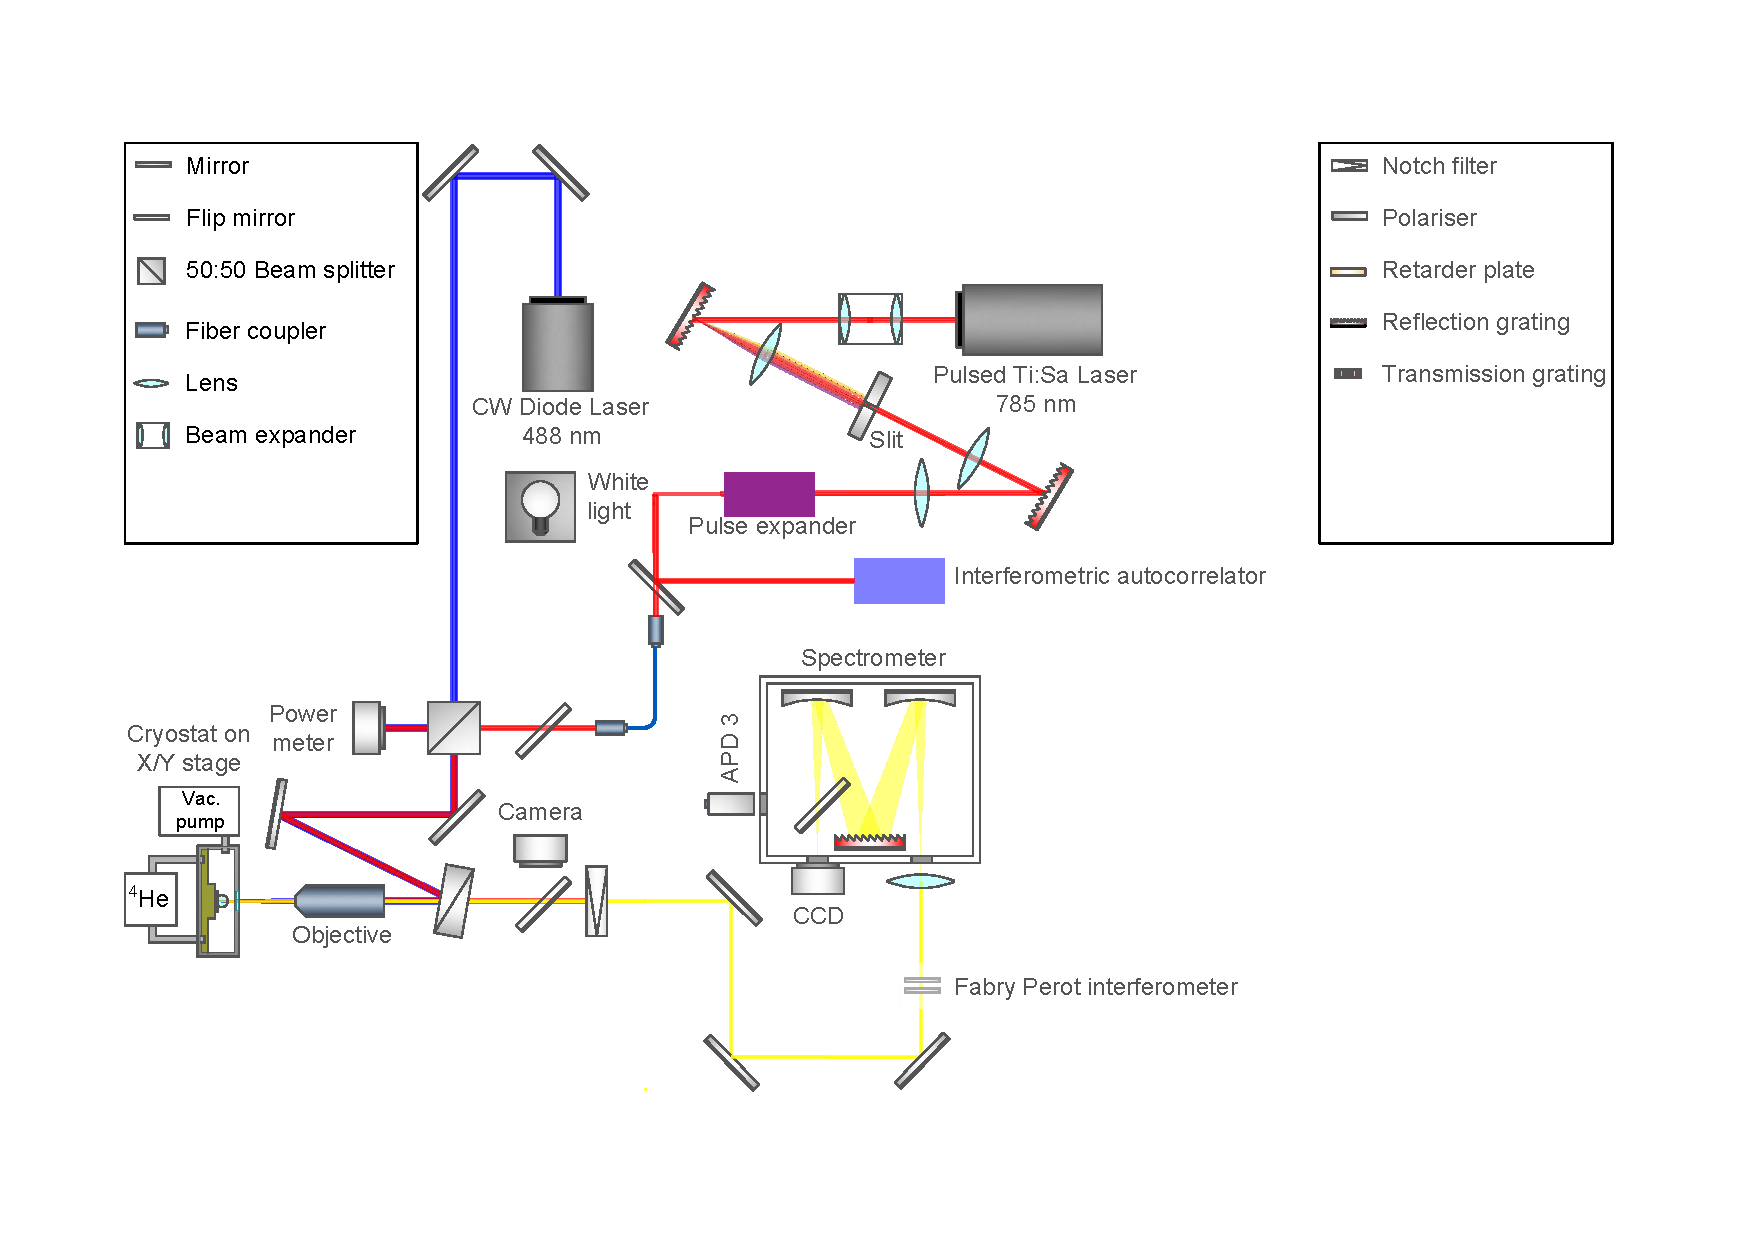
\includegraphics[width=1.1\linewidth]{figures/setup/Setup_flat}
	\caption[Complete experimental setup]{Complete experimental setup, which was used in order to quantify the chirp of the Ti:Sa Laser and resolve spectral emission of a quantum dot~\cite{schimpf_towards_2017}.}
	\label{fig:setupflat}
\end{figure}
